%%%%%%%%%%%%%%%%%%%%%%%%%%%%%%%%%%%%%%%%%
% Lachaise Assignment
% LaTeX Template
% Version 1.0 (26/6/2018)
%
% This template originates from:
% http://www.LaTeXTemplates.com
%
% Authors:
% Marion Lachaise & François Févotte
% Vel (vel@LaTeXTemplates.com)
%
% License:
% CC BY-NC-SA 3.0 (http://creativecommons.org/licenses/by-nc-sa/3.0/)
% 
%%%%%%%%%%%%%%%%%%%%%%%%%%%%%%%%%%%%%%%%%

%----------------------------------------------------------------------------------------
%	PACKAGES AND OTHER DOCUMENT CONFIGURATIONS
%----------------------------------------------------------------------------------------

\documentclass{article}
\usepackage{float}

%%%%%%%%%%%%%%%%%%%%%%%%%%%%%%%%%%%%%%%%%
% Lachaise Assignment
% Structure Specification File
% Version 1.0 (26/6/2018)
%
% This template originates from:
% http://www.LaTeXTemplates.com
%
% Authors:
% Marion Lachaise & François Févotte
% Vel (vel@LaTeXTemplates.com)
%
% License:
% CC BY-NC-SA 3.0 (http://creativecommons.org/licenses/by-nc-sa/3.0/)
% 
%%%%%%%%%%%%%%%%%%%%%%%%%%%%%%%%%%%%%%%%%

%----------------------------------------------------------------------------------------
%	PACKAGES AND OTHER DOCUMENT CONFIGURATIONS
%----------------------------------------------------------------------------------------

\usepackage{amsmath,amsfonts,stmaryrd,amssymb} % Math packages

\usepackage{enumerate} % Custom item numbers for enumerations

\usepackage[ruled]{algorithm2e} % Algorithms

\usepackage[framemethod=tikz]{mdframed} % Allows defining custom boxed/framed environments

\usepackage{listings} % File listings, with syntax highlighting
\lstset{
	basicstyle=\ttfamily, % Typeset listings in monospace font
}

%----------------------------------------------------------------------------------------
%	DOCUMENT MARGINS
%----------------------------------------------------------------------------------------

\usepackage{geometry} % Required for adjusting page dimensions and margins

\geometry{
	paper=a4paper, % Paper size, change to letterpaper for US letter size
	top=2.5cm, % Top margin
	bottom=3cm, % Bottom margin
	left=2.5cm, % Left margin
	right=2.5cm, % Right margin
	headheight=14pt, % Header height
	footskip=1.5cm, % Space from the bottom margin to the baseline of the footer
	headsep=1.2cm, % Space from the top margin to the baseline of the header
	%showframe, % Uncomment to show how the type block is set on the page
}

%----------------------------------------------------------------------------------------
%	FONTS
%----------------------------------------------------------------------------------------

\usepackage[utf8]{inputenc} % Required for inputting international characters
\usepackage[T1]{fontenc} % Output font encoding for international characters

\usepackage{XCharter} % Use the XCharter fonts

%----------------------------------------------------------------------------------------
%	COMMAND LINE ENVIRONMENT
%----------------------------------------------------------------------------------------

% Usage:
% \begin{commandline}
%	\begin{verbatim}
%		$ ls
%		
%		Applications	Desktop	...
%	\end{verbatim}
% \end{commandline}

\mdfdefinestyle{commandline}{
	leftmargin=10pt,
	rightmargin=10pt,
	innerleftmargin=15pt,
	middlelinecolor=black!50!white,
	middlelinewidth=2pt,
	frametitlerule=false,
	backgroundcolor=black!5!white,
	frametitle={Command Line},
	frametitlefont={\normalfont\sffamily\color{white}\hspace{-1em}},
	frametitlebackgroundcolor=black!50!white,
	nobreak,
}

% Define a custom environment for command-line snapshots
\newenvironment{commandline}{
	\medskip
	\begin{mdframed}[style=commandline]
}{
	\end{mdframed}
	\medskip
}

%----------------------------------------------------------------------------------------
%	FILE CONTENTS ENVIRONMENT
%----------------------------------------------------------------------------------------

% Usage:
% \begin{file}[optional filename, defaults to "File"]
%	File contents, for example, with a listings environment
% \end{file}

\mdfdefinestyle{file}{
	innertopmargin=1.6\baselineskip,
	innerbottommargin=0.8\baselineskip,
	topline=false, bottomline=false,
	leftline=false, rightline=false,
	leftmargin=2cm,
	rightmargin=2cm,
	singleextra={%
		\draw[fill=black!10!white](P)++(0,-1.2em)rectangle(P-|O);
		\node[anchor=north west]
		at(P-|O){\ttfamily\mdfilename};
		%
		\def\l{3em}
		\draw(O-|P)++(-\l,0)--++(\l,\l)--(P)--(P-|O)--(O)--cycle;
		\draw(O-|P)++(-\l,0)--++(0,\l)--++(\l,0);
	},
	nobreak,
}

% Define a custom environment for file contents
\newenvironment{file}[1][File]{ % Set the default filename to "File"
	\medskip
	\newcommand{\mdfilename}{#1}
	\begin{mdframed}[style=file]
}{
	\end{mdframed}
	\medskip
}

%----------------------------------------------------------------------------------------
%	NUMBERED QUESTIONS ENVIRONMENT
%----------------------------------------------------------------------------------------

% Usage:
% \begin{question}[optional title]
%	Question contents
% \end{question}

\mdfdefinestyle{question}{
	innertopmargin=1.2\baselineskip,
	innerbottommargin=0.8\baselineskip,
	roundcorner=5pt,
	nobreak,
	singleextra={%
		\draw(P-|O)node[xshift=1em,anchor=west,fill=white,draw,rounded corners=5pt]{%
		Question \theQuestion\questionTitle};
	},
}

\newcounter{Question} % Stores the current question number that gets iterated with each new question

% Define a custom environment for numbered questions
\newenvironment{question}[1][\unskip]{
	\bigskip
	\stepcounter{Question}
	\newcommand{\questionTitle}{~#1}
	\begin{mdframed}[style=question]
}{
	\end{mdframed}
	\medskip
}

%----------------------------------------------------------------------------------------
%	WARNING TEXT ENVIRONMENT
%----------------------------------------------------------------------------------------

% Usage:
% \begin{warn}[optional title, defaults to "Warning:"]
%	Contents
% \end{warn}

\mdfdefinestyle{warning}{
	topline=false, bottomline=false,
	leftline=false, rightline=false,
	nobreak,
	singleextra={%
		\draw(P-|O)++(-0.5em,0)node(tmp1){};
		\draw(P-|O)++(0.5em,0)node(tmp2){};
		\fill[black,rotate around={45:(P-|O)}](tmp1)rectangle(tmp2);
		\node at(P-|O){\color{white}\scriptsize\bf !};
		\draw[very thick](P-|O)++(0,-1em)--(O);%--(O-|P);
	}
}

% Define a custom environment for warning text
\newenvironment{warn}[1][Warning:]{ % Set the default warning to "Warning:"
	\medskip
	\begin{mdframed}[style=warning]
		\noindent{\textbf{#1}}
}{
	\end{mdframed}
}

%----------------------------------------------------------------------------------------
%	INFORMATION ENVIRONMENT
%----------------------------------------------------------------------------------------

% Usage:
% \begin{info}[optional title, defaults to "Info:"]
% 	contents
% 	\end{info}

\mdfdefinestyle{info}{%
	topline=false, bottomline=false,
	leftline=false, rightline=false,
	nobreak,
	singleextra={%
		\fill[black](P-|O)circle[radius=0.4em];
		\node at(P-|O){\color{white}\scriptsize\bf i};
		\draw[very thick](P-|O)++(0,-0.8em)--(O);%--(O-|P);
	}
}

% Define a custom environment for information
\newenvironment{info}[1][Info:]{ % Set the default title to "Info:"
	\medskip
	\begin{mdframed}[style=info]
		\noindent{\textbf{#1}}
}{
	\end{mdframed}
}
 % Include the file specifying the document structure and custom commands

%----------------------------------------------------------------------------------------
%	ASSIGNMENT INFORMATION
%----------------------------------------------------------------------------------------

\title{Warehouse Robot Synchronization Simulation} % Title of the assignment

\author{Boussaid Abderrazag & Mohamed Ben Hadj Nasr}
\date{University of Tunis El Manar --- Higher Institute of Computer Science \\ \today} % University, school and/or department name(s) and a date

%----------------------------------------------------------------------------------------

\begin{document}

\maketitle % Print the title

%----------------------------------------------------------------------------------------
%	INTRODUCTION
%----------------------------------------------------------------------------------------

\section*{Introduction} % Unnumbered section

This mini-project demonstrates a fundamental concept in concurrent programming: resource synchronization. It simulates multiple warehouse robots attempting to access a shared shelf, illustrating the problems that can occur without proper synchronization and how those problems can be solved using locks.

\section{The Problem: Race Conditions in Concurrent Access}

\subsection{Scenario Overview}

In the warehouse simulation, multiple robot threads simultaneously attempt to access a single shelf. Without proper synchronization, this creates a race condition - a situation where the behavior of the system depends on the relative timing of events, which can lead to unpredictable and undesirable outcomes.

\subsection{Specific Issues Observed}
When running the simulation without synchronization, the following problems occur:

\begin{itemize}
	\item Resource Corruption: Multiple robots might believe the shelf is available simultaneously.
	\item Conflicting Access: Robots attempt to use the shelf while another robot is already using it.
	\item Collision Risk: Physical robots would crash into each other at the shelf location.
	\item Inconsistent State: The shelf\_available and current\_robot variables are read and modified by multiple threads without coordination.
\end{itemize}

\begin{figure}[H]
	\centering
	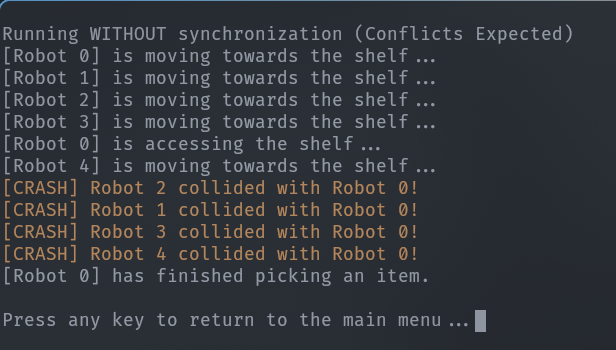
\includegraphics[width=0.7\textwidth]{./images/crash.png}
	\caption{showcase How robots crash}
	\label{fig:showcase-How-robots-crash}
\end{figure}

\subsection{Code Analysis of the Unsynchronized Implementation}

\begin{file}[Main.py]
	\begin{lstlisting}[language=Python]
def access_shelf_without_lock(robot_id):
    global shelf_available, current_robot
    if shelf_available:
        shelf_available = False
        current_robot = robot_id
        time.sleep(random.uniform(1.0, 2.0))
        shelf_available = True
        current_robot = None
\end{lstlisting}
\end{file}

The critical issue occurs in the sequence between checking if shelf\_available is True and setting it to False. If two robots check the condition almost simultaneously:

\begin{enumerate}
	\item Robot A checks shelf\_available (finding it True)
	\item Before Robot A sets shelf\_available = False, Robot B also checks shelf\_available (also finding it True)
	\item Both robots now believe they have exclusive access to the shelf
	\item Both robots proceed to access the shelf simultaneously, causing a collision
\end{enumerate}

This demonstrates a classic race condition where the outcome depends on the precise timing of thread execution.


\section{The Solution: Mutex Locks for Synchronization}
\subsection{Synchronization Technique: Mutex Lock}
The solution implements a mutex (mutual exclusion) lock using Python's threading.Lock(). A mutex ensures that only one thread can access a critical section of code at any given time, preventing race conditions.
\subsection{Implementation Details}

\begin{file}[Main.py]
	\begin{lstlisting}[language=Python]
def access_shelf_with_lock(robot_id):
    global shelf_available, current_robot
    time.sleep(random.uniform(0.5, 1.0))
    with lock:
        shelf_available = False
        current_robot = robot_id
        time.sleep(random.uniform(1.0, 2.0))
        shelf_available = True
        current_robot = None
\end{lstlisting}
\end{file}

The key improvements in this implementation are:

The ``with lock:`` statement creates a critical section that only one thread can enter at a time.
When a robot thread enters this section, it acquires the lock, preventing other robots from entering until it releases the lock.
The entire sequence of checking availability, marking the shelf as occupied, performing the task, and marking it as available again is protected within this critical section.
The lock is automatically released when the robot thread exits the with block, even if an exception occurs.

\subsection{How the Lock Resolves the Race Condition}
When Robot A acquires the lock:

\begin{enumerate}
	\item Robot A enters the critical section and sets shelf\_available = False
	\item Robot B attempts to acquire the lock but must wait
	\item Robot A completes its task, sets shelf\_available = True, and releases the lock
	\item Only then can Robot B acquire the lock and access the shelf
\end{enumerate}

This sequential access eliminates the possibility of collisions and ensures data consistency.

\begin{figure}[H]
	\centering
	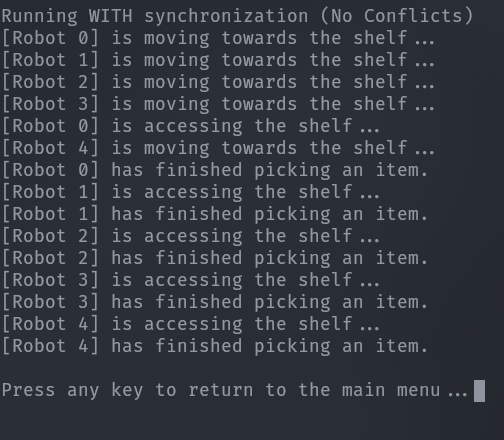
\includegraphics[width=0.6\textwidth]{./images/good_ending.png}
\end{figure}

\section{Technical Benefits and Considerations}
\subsection{Advantages of the Lock-Based Solution}

\begin{itemize}
	\item Deterministic Behavior: The system now behaves predictably regardless of thread timing.
	\item Data Integrity: Shared variables are protected from simultaneous access.
	\item Safety: In a physical implementation, robot collisions would be prevented.
	\item Simplicity: The threading.Lock provides a straightforward synchronization mechanism.
\end{itemize}
\end{document}
